\chapter{Designs} \label{appendix:designs} 

\section{Legenda} \label{appendix:legenda} 

In order to visualize the designs of the artifact, a standard UML notation is used. The
designs containing relationships adhere to the following definitions.

\begin{figure}[H]
  \centering
  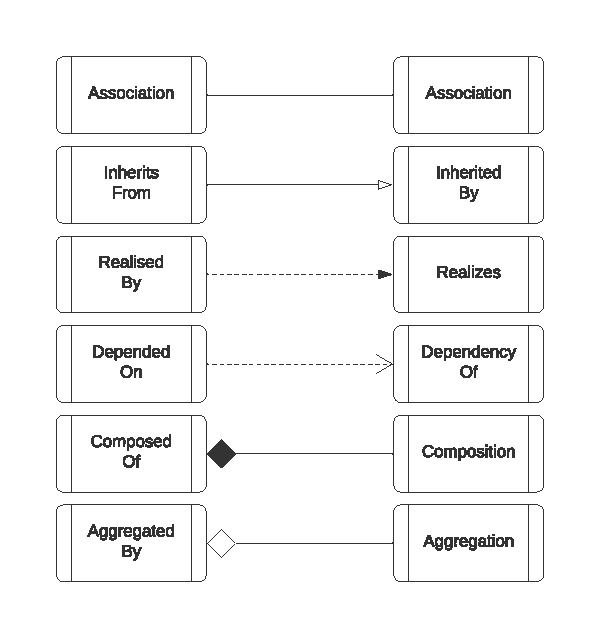
\includegraphics[width=1\textwidth]{Figures/class_diagram_legenda.pdf}
  \caption[Generic architecture]{UML notation}
  \label{fi:class_diagram_relationship_notation}
\end{figure}

\section{Generic design} \label{appendix:generic_design} 
\begin{figure}[H]
  \centering
  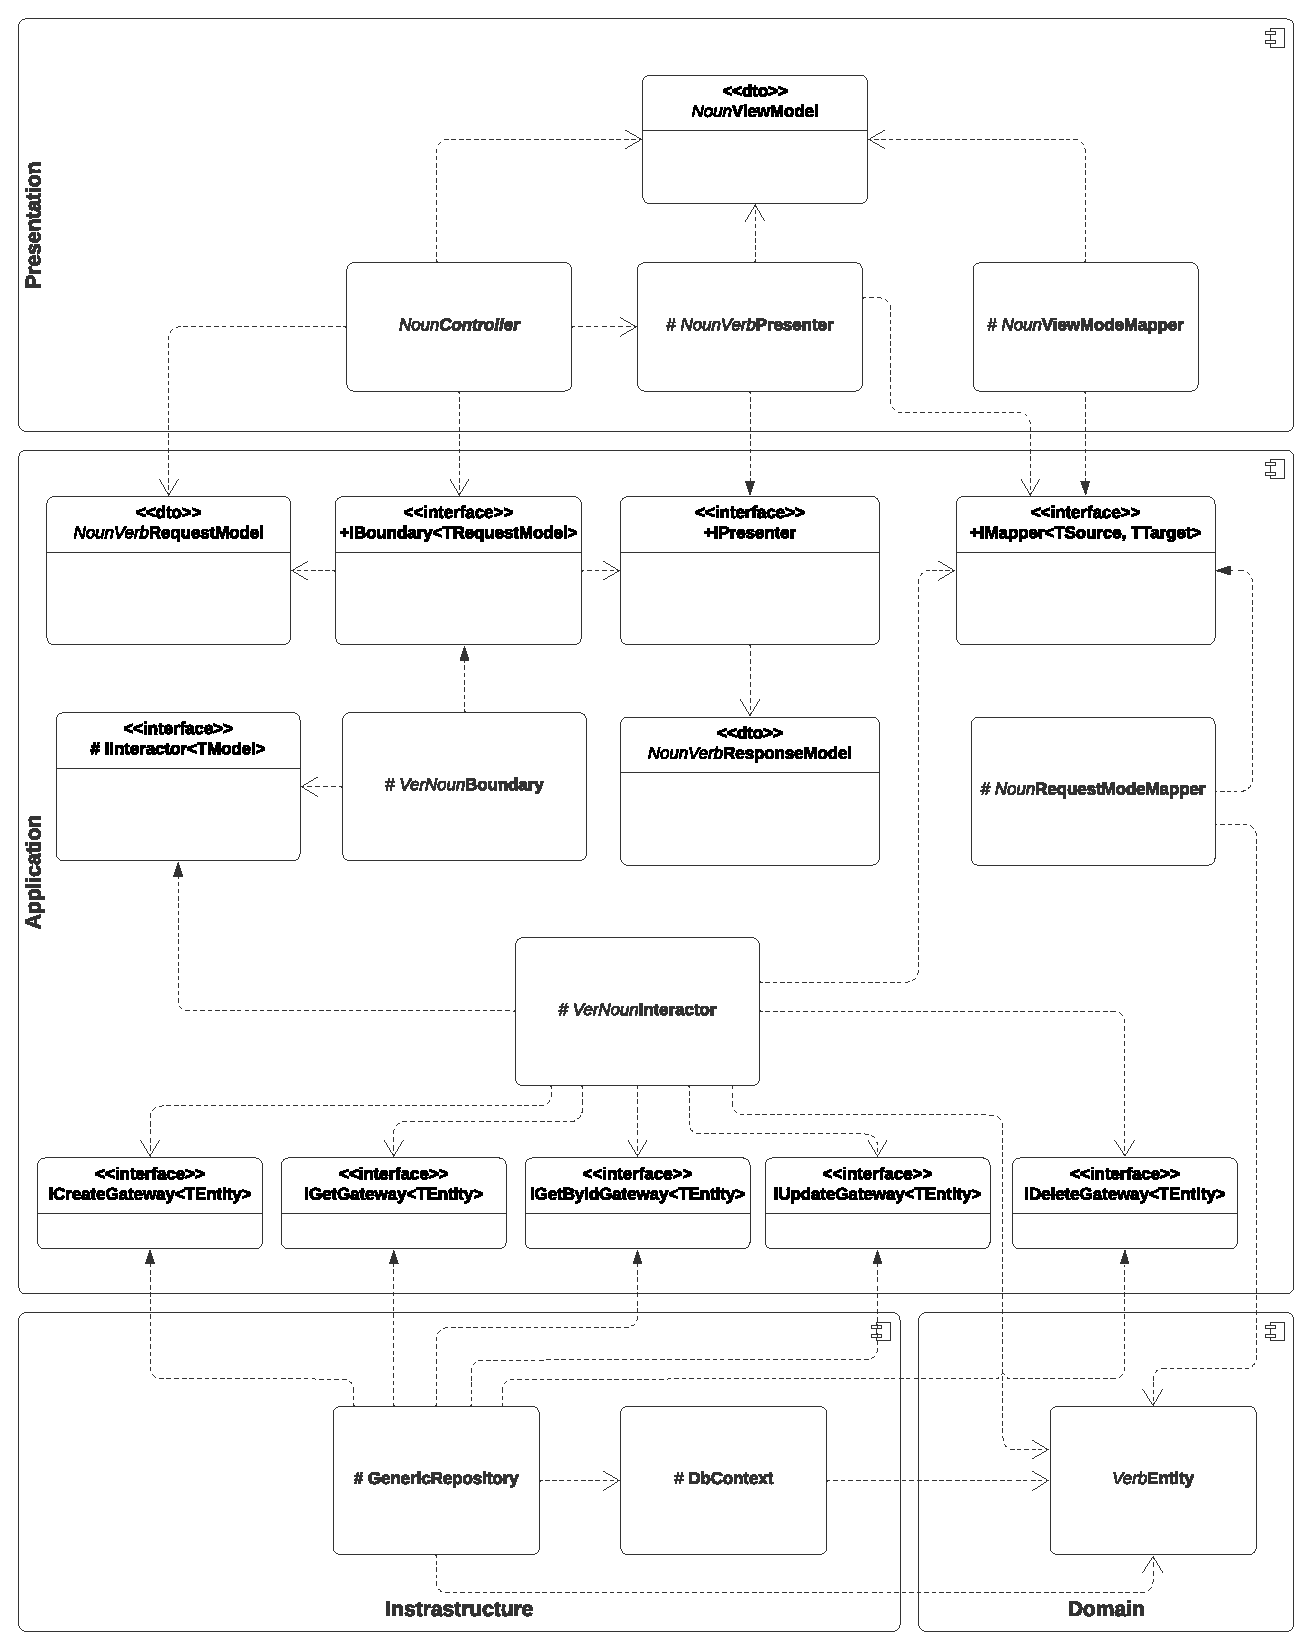
\includegraphics[width=1\textwidth]{Figures/classdiagram_generic_architecture.pdf}
  \caption[Generic architecture]{The Generic architecture of the artifacts}
  \label{fi:generic_design}
\end{figure}